\documentclass[11pt,a4]{article}
\usepackage{acl2010}
\usepackage{times}
\usepackage{url}
\usepackage{latexsym}
\usepackage{epsfig}
\usepackage{latexsym}
\usepackage[usenames]{color}
\usepackage{times} 
\usepackage{verbatim}
\usepackage{multirow}

\begin{document}

\author{David Jurgens\\
  University of California, Los Angeles\\
  Los Angeles, California, USA\\
  {\tt jurgens@cs.ucla.edu} \And
  Keith Stevens \\
  University of California, Los Angeles\\
  Los Angeles, California, USA\\
  {\tt kstevens@cs.ucla.edu}}

\title{
  HERMIT: Flexible Clustering for the SemEval-2 WSI Task}

\date{}

\maketitle

\begin{abstract}

A single word may have multiple unspecified meanings in a corpus.  Word sense
induction aims to discover these different meanings through word use, and
knowledge-lean algorithms attempt this without using external lexical resources.
We propose a new method for identifying the different senses that uses a
flexible clustering strategy to automatically determine the number of senses,
rather than predefining it.  We demonstrate the effectiveness using the
SemEval-2 WSI task, achieving competitive scores on both the V-Measure and
Recall metrics, depending on the parameter configuration.

\end{abstract}
  
\section{Introduction}

The Word Sense Induction task of SemEval 2010 compares several sense induction
and discrimination systems that are trained over a common corpus.  Systems are
provided with an unlabeled training corpus consisting of 879,807 contexts for
100 polysemous words, with 50 nouns and 50 verbs.  Each context
consists of several sentences that use a single sense of a target word, where at
least one sentence contains the word.  Systems must use the training corpus to
induce sense representations for the many word senses 
and then use those representations to produce sense labels for the same 100
words in unseen contexts from a testing corpus.

We perform this task by utilizing a distributional word space formed using
dimensionality reduction and a hybrid clustering method.  Our model is highly
scalable; the dimensionality of the word space is reduced immediately through a
process based on random projections.  In addition, an online part of our
clustering algorithm maintains only a centroid that describes an induced word
sense, instead of all observed contexts, which lets the model scale to much
larger corpora than those used in the SemEval-2 WSI task.

\section{The Word Sense Induction Model}
\label{sec:alg}

We perform word sense induction by modeling individual contexts in a high
dimensional word space.  
Word senses are induced by finding contexts which are similar and therefore
likely to use the same sense of the target word.  We use a hybrid clustering
method to group similar contexts. 

\subsection{Modeling Context}
\label{sec:context}

For a word, each of its contexts are represented by the words with which it
co-occurs.  We approximate this high dimensional co-occurrence space with the
Random Indexing (RI) word space model \cite{kanerva00random}.  RI represents the
occurrence of a word with an \emph{index vector}, rather than a set of
dimensions.  An index vector is a fixed, sparse vector that is orthogonal to all
other words' index vectors with a high probability; the total number of
dimensions in the model is fixed at a small value, e.g.\ 5,000.  Orthogonality
is obtained by setting a small percentage of the vector's values to $\pm1$ and
setting the rest to $0$.

A context is represented by summing the index vectors corresponding to the $n$
words occurring to the left and right of the polysemous word.  
Each occurrence of the polysemous word in the entire corpus is treated as a
separate context.
Contexts are represented by a compact first-order occurrence vector; using index
vectors to represent the occurrences avoids the computational overhead of other
dimensional reduction techniques such as the SVD.

\subsection{Identifying Related Contexts}
\label{sec:clustering}

Clustering separates similar context vectors into dissimilar clusters that
represent the distinct senses of a word.  We use an efficient hybrid of online
K-Means and Hierarchical Agglomerative Clustering (HAC) with a threshold.  The
threshold allows for the final number of clusters to be determined by data
similarity instead of having to specify the number of clusters.

The set of context vectors for a word are clustered using K-Means, which
assigns a context to the most similar cluster centroid.  If the nearest centroid
has a similarity less than the \emph{cluster threshold} and there are not $K$
clusters, the context forms a new cluster.  We define the similarity between
contexts vectors as the cosine similarity.

Once the corpus has been processed, clusters are repeatedly merged using HAC
with the average link criteria, following \cite{pedersen97distinguishing}.
Average link clustering defines cluster similarity as the mean cosine similarity
of the pairwise similarity of all data points from each cluster.  Cluster
merging stops when the two most similar clusters have a similarity less than the
cluster threshold.  Reaching a similarity lower than the cluster threshold
signifies that each cluster represents a distinct word sense.  

\subsection{Applying Sense Labels}

Before training and evaluating our model, all occurrences of the 100 polysemous
words were stemmed in the corpora.  Stemming was required due to a polysemous
word being used in multiple lexical forms, e.g.\ plural, in the corpora.  By
stemming, we avoid the need to combine contexts for each of the distinct word
forms during clustering.

After training our WSI model on the training corpus, we process the test corpus
and label the context for each polysemous word with an induced sense.  
%
Each test context is labeled with the name of the cluster whose centroid has the
highest cosine similarity to the context vector.
%
We represent the test contexts in the same method used for training; index
vectors are re-used from training.


\section{Evaluation and Results}

The WSI task evaluated the submitted solutions with two methods of
experimentation: an unsupervised method and a supervised method.  The
unsupervised method is measured according to the V-Measure and the F-Score.  The
supervised method is measured using recall.

\subsection{Scoring}

The first measure used is the V-Measure \cite{rosenberg07vmeasure},
which compares the clusters of target contexts to word classes.  This measure
rates the homogeneity and completeness of a clustering solution.  Solutions that
have word clusters formed from one word class are homogeneous; completeness
measures the degree to which a word class is composed of target contexts
allocated to a single cluster.

The second measure, the F-Score, is an extension from information retrieval
and provides a contrasting evaluation metric by using a different
interpretation of homogeneity and completeness.  For the F-Score, the precision
and recall of all possible context pairs are measured, where a word class has
the expected context pairs and a provided solution contains some word pairs that
are correct and others that are unexpected.  The F-Score tends to discount
smaller clusters and clusters that cannot be assigned to a word class
\cite{manandhar09semeval}.

\subsection{Parameter Tuning}

Previous WSI evaluations provided a test corpus, a set of golden sense labels,
and a scoring mechanism, which allowed models to do parameter tuning prior to
providing a set of sense labels.  The SemEval 2010 task provided a trial corpus
that contains contexts for four verbs that are not in the evaluation corpus,
which can be used for training and testing.  The trial corpus also came with a
set of golden sense assignments.  No golden standard was provided for the
training or test corpora, which limited any parameter tuning.

HERMIT exposes three parameters: cluster threshold, the maximum number of
clusters and the window size for a context.  An initial analysis from the trial
data showed that the window size most affected the scores; small window sizes
resulted in higher V-Measure scores, while larger window sizes maximized the
F-Score.  Because
contexts are represented using only first-order features, a smaller window size
should have less overlap, which potentially results in a higher number of
clusters.  We opted to maximize the V-Measure score by using a window size of
$\pm 1$.

Due to the limited number of training instances, our precursory analysis with
the trial data did not show significant differences for the remaining two
parameters; we arbitrarily selected a clustering threshold of {\bf .15} and a
maximum of {\bf 15} clusters per word without any parameter tuning.

After the release of the testing key, we performed a post-hoc analysis to
evaluate the effects of parameter tuning on the scores.  We include two
alternative parameter configurations that were optimized for the F-Score
(HERMIT-F) and the supervised evaluations (HERMIT-S).  The HERMIT-F variation
used a threshold of 0.85 and a window size of $\pm 10$ words.  The HERMIT-S
variation used a threshold of 0.85 and a window size of $\pm 1$ words.  We did
not vary the maximum number of clusters, which was set at 15.

For each evaluation, we provide the scores of seven systems: the three HERMIT
configurations, the highest and lowest scoring submitted systems, the Most
Frequent Sense (MFS) baseline, and a Random baseline provided by the evaluation
team.  We provide the scores for each experiment when evaluating all words,
nouns, and verbs.  We also include the system's rank relative to all submitted
systems and the average number of senses generated for each system; our
alternative HERMIT configurations are given no rank.


\subsection{Unsupervised Evaluation}


\begin{table}[htb]
  \small
  \center
  \begin{tabular}{| l | ccccc | }
    \hline
    System & All & Nouns & Verbs & Rank & Senses \\
    \hline
    HERMIT-S & 16.2 & 16.7 & 15.3 & & 10.83 \\
    HERMIT   & 16.1 & 16.7 & 15.6 & 1 & 10.78 \\
    Random   & 4.4  & 4.6  & 4.1 & 18 & 4.00 \\
    HERMIT-F & 0.015 & 0.008 & 0.025 & & 1.54 \\
    MFS      & 0.0  & 0.0 & 0.0 & 27 & 1.00 \\
    LOW      & 0.0  & 0.0 & 0.1 & 28 & 1.01 \\
    \hline
  \end{tabular}
  \caption{V-Measure for the unsupervised evaluation}
  \label{tab:evaluation-v}
\end{table}

\begin{table}[htb]
  \small
  \center
  \begin{tabular}{| l | ccccc | }
    \hline
    System & All & Nouns & Verbs & Rank & Senses \\
    \hline
    MFS      & 63.4 & 57.0 & 72.7 & 1 & 1.00 \\
    HIGH     & 63.3 & 57.0 & 72.4 & 2 & 1.02 \\
    HERMIT-F & 62.1 & 56.7 & 69.9 & & 1.54 \\
    Random   & 31.9 & 30.4 & 34.1 & 25 & 4.00 \\
    HERMIT   & 26.7 & 30.1 & 24.4 & 27 & 10.78 \\
    HERMIT-S & 26.5 & 23.9 & 30.3 & & 10.83 \\
    LOW      & 16.1 & 15.8 & 16.4 & 28 & 9.71 \\
    \hline
  \end{tabular}
  \caption{F-Scores for the unsupervised evaluation}
  \label{tab:evaluation-f}
\end{table}


The unsupervised evaluation considers a golden sense labeling to be word classes
and a set of induced word senses as clusters of target contexts
\cite{manandhar09semeval}.  
%
Tables \ref{tab:evaluation-v} and \ref{tab:evaluation-f} display the results for
the unsupervised evaluation when measured according to the V-Measure and the
F-Score, respectively.  Our system provides the best V-Measure of all submitted
systems for this evaluation.  This is in part due to the average number of
senses our system generated (10.78), which favors more homogenous clusters.
Conversely, this configuration does poorly when measured by F-Score, which tends
to favor systems that generate fewer senses per word.  

When configured for the F-Score, HERMIT-F performs well; this configuration
would have ranked third for the F-Score if it had been submitted.  However, its
performance is also due to the relatively few senses per word it generates,
1.54.  The inverse performance of both optimized configurations is reflective of
the contrasting nature of the two performance measures.

\subsection{Supervised Evaluation}

\begin{table}[tbh]
  \center
  \small
  \begin{tabular} { | l | cccc |}
      \hline
      System & All & Noun & Verb & Rank \\
      \hline
      HIGH & 62.44 & 59.43 & 66.82 & 1 \\
      MFS & 58.67 & 53.22  & 66.620 & 15 \\
      HERMIT-S & 58.48 & 54.18 & 64.78 & \\
      HERMIT & 58.34 & 53.56 & 65.30 & 17 \\
      Random & 57.25 & 51.45 & 65.69 & 19 \\
      HERMIT-F & 56.44 & 53.00 & 61.46 & \\
      LOW & 18.72 & 1.55 & 43.76 & 28 \\
      \hline
  \end{tabular}
  \caption{Supervised recall for the 80/20 split}
  \label{tab:evaluation-80}
\end{table}

\begin{table}[tbh]
  \center
  \small
  \begin{tabular} { | l | cccc |}
      \hline
      System & All & Noun & Verb & Rank \\
      \hline
      HIGH & 61.96 & 58.62 & 66.82 & 1 \\
      MFS & 58.25 & 52.45 & 67.11 & 12 \\
      HERMIT & 57.27 & 52.53 & 64.16 & 18 \\
      HERMIT-S & 57.10 & 52.76 & 63.46 &  \\
      Random & 56.52 & 50.21 & 65.73 & 20 \\
      HERMIT-F & 56.18 & 52.26 & 61.88 & \\
      LOW & 18.91 & 1.52 & 44.23 & 28 \\
      \hline
  \end{tabular}
  \caption{Supervised recall for the 60/40 split}
  \label{tab:evaluation-60}
\end{table}

The supervised evaluation simulates a supervised Word Sense Disambiguation (WSD)
task.  The induced sense labels for the test corpus are split such that the
first set is used for mapping induced senses to golden senses and the remaining
sense labels are treated as sense labels provided by a WSD system, which allows
for evaluation.  Five splits are done at random to avoid any biases created due
to the separation of the mapping corpus and the evaluation corpus; the resulting
score for this task is the average recall over the five divisions.  Two sets of
splits were used for evaluation: one with 80\% of the senses as the mapping
portion and 20\% as the evaluation portion and one with 60\% as the mapping
portion corpus and 40\% for evaluation.

The results for the 80/20 split and 60/40 split are displayed in tables
\ref{tab:evaluation-80} and \ref{tab:evaluation-60}, respectively.  In both
supervised evaluations, our submitted system does moderately well.  In both
cases it outperforms the Random baseline and does almost as well as the MFS
baseline.  The submitted system outperforms the Random baseline and approaches
the MFS baseline for the 80/20 split. The HERMIT-S version, which is optimized
for this task, provides similar results.

\section{Discussion}
\begin{figure}
  \vspace{-1mm}
  \center 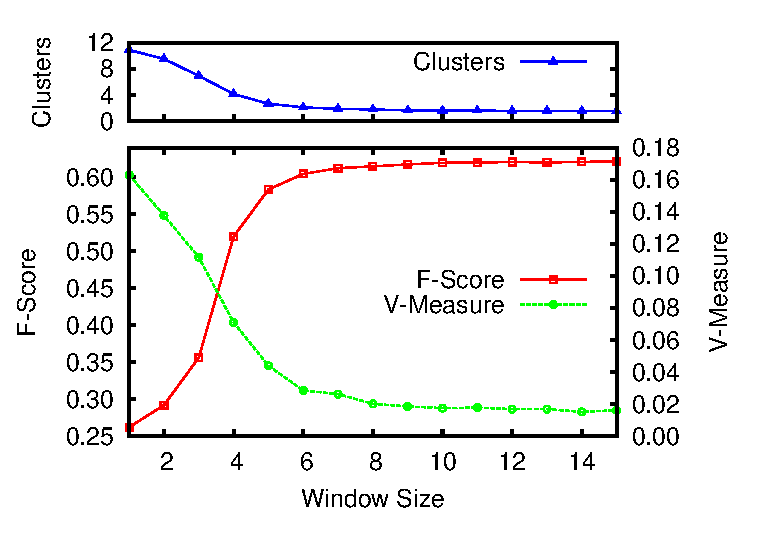
\includegraphics[width=.5\textwidth]{figures/hermit-score-comparison.eps}
  \vspace{-10mm}
  \caption{
    A comparison for F-Score and V-Measure for different window sizes.
    Scores are an average using thresholds of 0.15, 0.55 and 0.75.}
  \label{fig:algorithm} 
  \vspace{-1mm}
\end{figure}

The HERMIT system is easily configured to achieve close to state of the art
performance for either evaluation measure on the unsupervised benchmark.  This
reconfigurability allows the algorithm to be tuned for producing a few coarse
senses of a word, or many finer-grained senses.  

We further investigated the performance with respect to the window size
parameter on both measures.  Since each score can be effectively optimized
individually, we considered whether both scores could be maximized concurrently.
Figure \ref{fig:algorithm} presents the impact of the window size on both
measures using an average of three threshold parameter configurations.

The analysis of both measures indicates that reasonable performance can be
obtained from using a slightly larger context window.  For example, a window
size of 4 has an average F-Score of 52.4 and V-Measure of 7.1.  Although this
configuration produces scores lower than the optimized versions, its performance
would have ranked 12th according to V-Measure and 15th for F-Score.  These
scores are consistent with the median performance of the submitted systems and
offer a middle ground should a HERMIT user want a compromise between many
fine-grained word senses and a few coarse-grained word senses.

\section{Conclusion}

We have shown that our model is a highly flexible and tunable Word Sense
Induction model.  Depending on the task, it can be optimized to generate a set
of word senses that range from being broad and representative to highly
refined.
Furthermore, we demonstrated a balanced performance setting for both measures for
when parameter tuning is not possible.
The model we submitted and presented is only one possible configuration
available, and in the future we will be exploring the effect of other context
features, such as syntactic structure in the form of word ordering
\cite{sahlgren08permutations} or dependency parse trees, %
\cite{pado07dependency}, and other clustering algorithms.  Last, this model is
provided as part of the S-Space Package \cite{jurgens10sspace}, an open 
source toolkit for word space algorithms.


\bibliographystyle{acl}
\bibliography{semeval_2010}

\end{document}
